\chapter{Architektur}

	Beim hier verwendeten Entscheidungstemplate handelt es sich um das "`IBM UMF Template for Decision Log"'\cite{hand_ibm_2008}.
	
	\section{Erweiterung CDAR}
		Im folgenden werden die Möglichkeiten beschrieben, wie \eeppi\ an das CDAR angebunden werden soll.
		
		\decision{
			\decisionHeader{1}{Erweiterung CDAR/Integration}{Integration}{Architektur design}
		}{
			\decisionContent{}
			{In welcher Art soll \eeppi\ mit dem CDAR integriert werden?}
			{Die CDAR login API erlaubt das Bauen eines SSO über mehrere Applikationen hinweg}
			{Möglichst grosse Unabhängigkeit vom CDAR, möglichst einfaches Handling für den Benutzer}
			{
				\begin{description}
					\item[Lose Kopplung, keine UI Integration]
					\eeppi\ benutzt die CDAR API und den Login-Mechanismus und besitzt eine eigene Server- sowie UI-Komponente.
					\begin{description}
						\item[Vorteile] Keine Anpassungen an CDAR, \eeppi\ ist Unabhängig vom CDAR und könnte auch mit einer andern Applikation als das CDAR gekoppelt werden, SSO für Benutzer
						\item[Nachteile] Benutzer müssen zwei Applikationen nutzen (andere URL als CDAR)
					\end{description}
					
					\item[Lose Kopplung, CDAR UI erweitern]
					\eeppi\ benutzt die CDAR API und den Login-Mechanismus, besitzt eine eigene Serverkomponente und erweitert die UI Komponente des CDAR.			
					\begin{description}
						\item[Vorteile] Nur eine Applikation für Benutzer
						\item[Nachteile] CDAR UI muss angepasst werden, \eeppi\ ist vom CDAR abhängig
					\end{description}
					
					\item[Serverkomponente ersetzen, keine UI Integration]
					\eeppi\ bildet eine gemeinsame neue Serverkomponente, die diejenige des CDAR ersetzt. Die CDAR UI Komponente wird weiterverwendet. 
					Die \eeppi\ spezifische Funktionalität sind in einer eigenen UI Komponente untergebracht.
					\begin{description}
						\item[Vorteile] Einheitlichen Unterbau für CDAR und \eeppi, nur eine Schnittstelle, Serverkomponente und Persistence
						\item[Nachteile] Sehr aufwändig, da die CDAR Server Komponente viel zu ersetzende Logik beinhaltet, Benutzer müssen zwei Applikationen nutzen, \eeppi\ ist vom CDAR abhängig
					\end{description}
					
					\item[Serverkomponente ersetzen, CDAR UI erweitern]
					\eeppi\ bildet eine gemeinsame neue Serverkomponente, die diejenige des CDAR ersetzt. Die \eeppi\ Funktionalitäten werden in das CDAR UI integriert.
					\begin{description}
						\item[Vorteile] Einheitlichen Unterbau für CDAR und \eeppi, nur eine Schnittstelle, Serverkomponente und Persistence, nur eine Applikation für Benutzer
						\item[Nachteile] Sehr aufwändig, da die CDAR Server Komponente viel zu ersetzende Logik beinhaltet, \eeppi\ ist vom CDAR abhängig werden.
					\end{description}
				\end{description}
			}
			{}
			{}
			{}
			{"`Server Technologie"', "`Tier Architektur"'}
		}
		

	\section{Architekturübersicht}
	
	
	\section{Tier-Architektur}
		Aufgrund der Einschränkung von Technologie und den existierenden Komponenten des CDAR's stehen drei mögliche Tier-Architekturen zur Auswahl.
		Die hier verwendeten Begriffe stützen sich auf von Prof. Dr. Zimmermann verwendete Begriffe in der HSR Vorlesung "`Application Architecture"'\cite{prof._dr._zimmerman_layers_20144}.		
		
		\begin{figure}[H]
			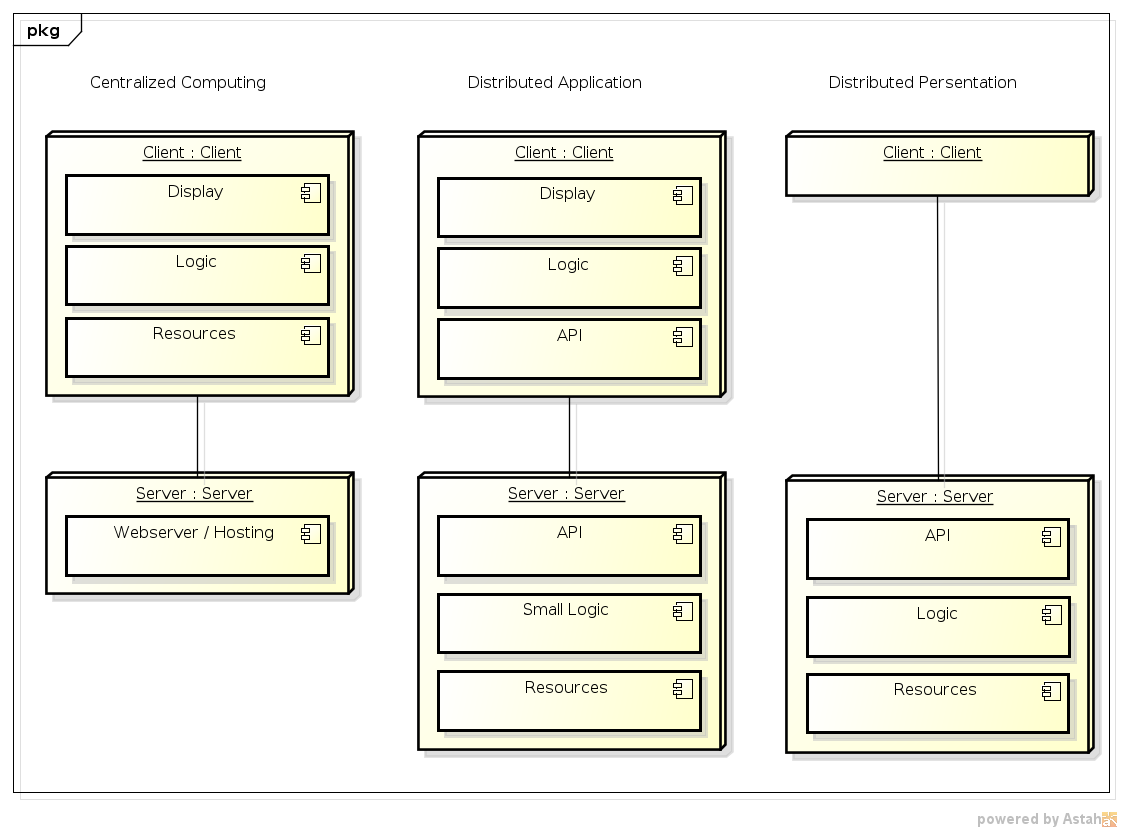
\includegraphics[width=\textwidth]{architecture/media/img/tierArchitecture.png}
			\centering
			\caption{Architektur Varianten}
			\label{fig:tierArchitecture}
		\end{figure}
		\begin{description}
			\item[1-Tier Structure: Centralized Computing (Client-only Application)]
				Die Serverkomponente übernimmt lediglich das Ausliefern einer WebApp. 
				Die WebApp bezieht die Daten direkt aus externen Schnittstellen. 
				Persistenz findet dezentral auf dem Client statt in Form von File Persistence oder 
				Persistence durch das Framework (z.B. HTML5 Storage).
				
			\item[2-Tier Structure: Distributed Application (Single Page App)]
				Die Serverkomponente übernimmt Persistenz sowie minimale Logik (z.B. Login).
				Presentation und Logik werden von der Client Komponente übernommen.
				
			\item[2-Tier Structure: Distributed Presentation]
				Persistenz, Logik und Presentation werden vom Server übernommen.
				Die Presentation wird fertig aufbereitet an den Client gesendet (z.B. HTML Page).
				Es gibt keine aktiven Komponenten auf dem Client ausser asyncron nachladenden Skripten.
				
		\end{description}
	
		\decision{
			\decisionHeader{1}{Tier Architektur}{Architektur}{Architektur design}
		}{
			\decisionContent{Distributed Application (Single Page Application)}
			{Welche Tier Architektur soll für \eeppi\ gewählt werden?}
			{}
			{Möglichst lose Kopplung \& hohe Flexibilität auch für zukunftüge, auf \eeppi\ und CDAR aufbauende Applikationen}
			{"`Centralized Computing"', "`Distributed Presentation"'}
			{"`Distributed Application"' ermöglicht, die bestehende Serverlogik des CDAR zu nutzen, 
				eine Serverseitige (zentralisierte) Persistenz anzubieten sowie dem Benutzer eine schnelle und unabhängige Applikation zur Verfügung zu stellen, 
				die die Rechenleistung des Clients beansprucht, sodass der Server und dessen Kosten schlank gehalten werden können.
				Da die App vom Server ausgeliefert wird, kann sie zentral von dort aus verwaltet, gewartet und kontrolliert werden.}
			{}
			{}
			{}
		}